% !TeX root = ../main.tex
\section{Design}
\label{sec:overview}
\label{sec:method}
Figure~\ref{fig:overview} shows how MECC connects an offline residency plan to the serving path.
The planner uses recorded expert selections, model dimensions, and HBM/CPU budgets to set capacities and initial resident IDs for each layer.
The loader places these experts in HBM and CPU memory.
HDD keeps the full set of expert weights as backing storage.
Together, the capacities and resident IDs define the cache state at deployment.

During inference, the router's selected IDs enter the cache for their layer.
A lookup identifies the source of each expert and updates HBM and CPU residency under that layer's fixed capacities.
Figure~\ref{fig:overview} shows two possible sources: $e_2$ is resident in CPU memory, while $e_6$ needs an HDD read.
Promoting $e_2$ frees its CPU slot, which can retain the expert displaced from HBM.
The delivery path brings each requested weight to the GPU and completes its transfer before execution.

The updated HBM and CPU resident sets carry into later tokens and requests.
An expert ID belongs to a particular layer, so the same ID in another layer denotes a different weight block.
Requests update only the accessed layer's state; other layers keep their residents.
This lets serving demand change the initial placement while preserving the capacities assigned by the planner.

\subsection{Expert Planner}
\label{sec:expert_planner}
\begin{figure}[H]
\centering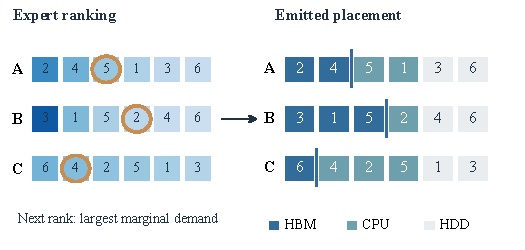
\includegraphics[width=\columnwidth]{figures/fig04_compile_frontiers.pdf}
\par\nointerlineskip
\caption{Initial placement across layers A--C. Circled entries are the next uncovered experts; shared HBM/CPU budgets set the cuts in each ranked list.}
\label{fig:compile}
\end{figure}

Consider $L$ MoE layers with $N_\ell$ experts per layer.
For the routed pools considered here, experts have equal size $s$ and layers use the same top-$k$, so each slot has the same capacity cost across layers.

Primary expert-residency budgets $B_{\mathrm H}$ and $B_{\mathrm C}$ provide $S_{\mathrm H}=\lfloor B_{\mathrm H}/s\rfloor$ HBM slots and $S_{\mathrm C}=\lfloor B_{\mathrm C}/s\rfloor$ CPU slots.
Physical host usage includes CPU residents, GPU-weight mirrors, and staging buffers.

Calibration orders experts by selection counts.
The analysis collects selected expert IDs separately for each layer.
Let $\pi_\ell(r)$ denote the local ID at rank $r$ in layer $\ell$.
Expert ID breaks equal-count ties.
Zero-count IDs follow observed experts in ID order.
The planner therefore compares demand across layers while preserving a separate expert list for each layer.
A log-count versus log-rank regression supplies $\alpha_\ell$ as the negative slope over positive counts.
The rank model smooths the observed selection frequencies for allocation scoring:
\begin{equation}
q_{\ell,r}=\frac{r^{-\alpha_\ell}}{\sum_{j=1}^{N_\ell}j^{-\alpha_\ell}}.
\end{equation}
Here $q_{\ell,r}$ is conditional selection mass within layer $\ell$, with unit sum.
Equal top-$k$ makes this mass comparable across layers.
Counts determine which expert occupies each rank; the rank model supplies the allocation scores.

Figure~\ref{fig:compile} shows the HBM and CPU cuts in those lists.
Capacities satisfy $\sum_\ell K_{\mathrm H,\ell}\le S_{\mathrm H}$, $\sum_\ell K_{\mathrm C,\ell}\le S_{\mathrm C}$, and $K_{\mathrm H,\ell}+K_{\mathrm C,\ell}\le N_\ell$.
The adaptive scan reserves one slot per layer in each fast tier, then distributes the remaining slots by marginal coverage.
The reservation accounts for $L$ slots in each tier before the remaining allowance is distributed.

The scan first assigns HBM slots.
At each step, it chooses the layer with the largest next-rank score:
\begin{equation}
\Delta_\ell=q_{\ell,K_{\mathrm H,\ell}+1}.
\end{equation}
CPU allocation continues from the first ranks beyond each HBM cut.
Its next candidate has score
\begin{equation}
\Delta^{\mathrm C}_\ell=q_{\ell,K_{\mathrm H,\ell}+K_{\mathrm C,\ell}+1}.
\label{eq:cpu_marginal}
\end{equation}
The HBM offset directs CPU slots to experts beyond those already selected for the GPU.
An eligible layer has an uncovered expert within its local list.
The scan compares these candidates, assigns one slot, and advances the selected layer's cut.
Every allocation exposes a new next-rank candidate in that layer.
Layer ID breaks score ties, and expert ID breaks count ties.
The direct scan takes $O(L(S_{\mathrm H}+S_{\mathrm C}))$ time after sorting.
Its score is the additional within-layer selection mass covered by the next slot.
Sorting the layer-local lists takes $O(\sum_\ell N_\ell\log N_\ell)$ time and runs once before deployment.

The expert planner serializes a residency plan: model dimensions, expert size, capacity arrays, and ranked layer-local IDs.
For layer $\ell$, ranks $1$ through $K_{\mathrm H,\ell}$ enter HBM.
Ranks $K_{\mathrm H,\ell}+1$ through $K_{\mathrm H,\ell}+K_{\mathrm C,\ell}$ enter the CPU resident set.
All other ranks remain available from the backing store.
The JSON plan is the deployment artifact consumed by the loader.
The loader constructs a cache for each layer from the corresponding IDs and capacities.
The capacity arrays remain fixed during serving.
Changing task demand updates the residents through online admission.

\subsection{Expert Retention}
\label{sec:expert_retention}
Each layer maintains two ordered sets, from most-recently used (MRU) to least-recently used (LRU).
Their concatenation places HBM residents before CPU residents.
The two primary sets contain distinct expert IDs.
The ordering describes recency across both managed tiers.
An HBM hit moves its expert to HBM MRU.
A CPU hit removes its host entry and promotes it to HBM MRU.
The evicted GPU LRU expert then becomes CPU MRU.
HDD retains the backing weights for every expert.
The cold payload comes from a completed read or a pending read resolved at consumption.
It enters HBM MRU and follows the same demotion rule as a CPU promotion.
If this admission exceeds the CPU capacity, the CPU LRU entry is removed.
The backing store supplies that expert again when a later request misses both tiers.

\begin{figure}[H]
\centering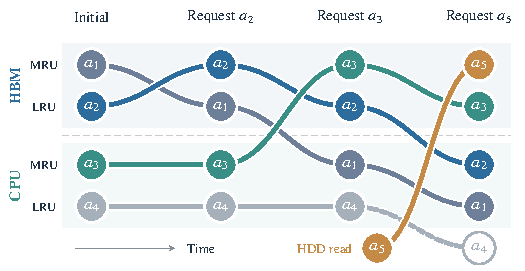
\includegraphics[width=\columnwidth]{figures/fig05_residency_cases.pdf}
\par\nointerlineskip
\caption{Expert recency across three requests. Colored paths track each expert; vertical order in each tier runs from MRU to LRU.}
\label{fig:retention}
\end{figure}
Figure~\ref{fig:retention} starts with HBM $[a_1,a_2]$ and CPU $[a_3,a_4]$.
Request $a_2$ gives HBM $[a_2,a_1]$.
Request $a_3$ then promotes $a_3$ and demotes $a_1$, producing HBM $[a_3,a_2]$ and CPU $[a_1,a_4]$.
Finally, $a_5$ enters HBM, $a_2$ becomes CPU MRU, and $a_4$ leaves CPU LRU.
The final lists are $[a_5,a_3]$ and $[a_2,a_1]$.

Each GPU resident carries a host mirror.
The implementation stores device weights and their host tensor together in the GPU entry.
On promotion, the CPU resident's host tensor continues as the promoted expert's mirror.
The released slot is a logical CPU residency entry.
The demoted expert's existing mirror becomes the new resident named by that entry.
This exchange retains the demoted weights through a metadata update and saves a device-to-host copy.

Mirrors and CPU residents serve different roles.
A mirror supports an expert currently assigned to HBM; a CPU resident supplies an expert outside the HBM set.
For equal-size blocks and full resident sets, their steady host payload is $s\sum_\ell(K_{\mathrm H,\ell}+K_{\mathrm C,\ell})$.
Pending reads and staging buffers add to this payload.
Deployment sizing includes these allocations alongside the primary CPU capacity.

The ordered maps support lookup and recency updates in expected constant time.
A CPU hit consumes one CPU entry before admitting the requested expert to HBM.
A cold access introduces a new resident and may remove the CPU tail.
After each access, the primary sets respect their assigned capacities.
Active tensor references extend the lifetime of weights through expert execution.

\subsection{Online Execution}
\label{sec:weight_delivery}
Serving requests update the initial state through the same access rules.
When a task selects different experts, its first accesses admit them to HBM.
Subsequent demotions place them at CPU MRU, while older CPU entries move toward replacement.
HBM hits refresh recency directly.
The updated state survives the end of a prompt and serves later requests on the same model instance.

For each MoE layer, the wrapper evaluates the gate and groups token rows by selected expert.
The loader resolves each layer-local expert ID through the memory tiers.
The expert kernel processes its assigned rows.
Gate weights scale the outputs before accumulation into the layer result.
The gate continues to determine expert selection and mixture weights.

During prefill, the loader submits reads for the selected experts absent from memory.
Each read is resolved when its expert reaches consumption.
Figure~\ref{fig:delivery} shows resident work overlapping a pending read for another selected expert.

\begin{figure}[H]
\centering% Illustrative prefill schedule. Coordinates express dependency order, not measured time.
\begin{tikzpicture}[x=1pt,y=1pt,>=Stealth,
  every node/.style={font=\fontsize{7}{7.7}\selectfont,inner sep=0pt}]
\path[use as bounding box] (0,0) rectangle (250,129);
\begin{scope}[yshift=-4pt]
\definecolor{delBlue}{HTML}{326C9B}
\definecolor{delTeal}{HTML}{6D9FAD}
\definecolor{delOrange}{HTML}{C78D51}
\definecolor{delInk}{HTML}{253645}
\node[anchor=west,text=delInk,font=\fontsize{7.3}{8}\selectfont\bfseries]
  at (3,131) {Selected experts: $a_1$ in HBM, $a_5$ on HDD};
\draw[->,draw=delInk!70,line width=.55pt] (63,120) -- (237,120);
\node[anchor=east,text=delInk] at (250,120) {time};

% The same resource lanes are used in both schedules.
\foreach \bottom/\title/\io/\gpu in {67/Serial/98/79,12/MECC/43/24}{
  \draw[delInk!40,line width=.5pt] (2,\bottom) rectangle (248,\bottom+48);
  \fill[delInk!3] (62,\io-7) rectangle (216,\io+7);
  \fill[delInk!3] (62,\gpu-7) rectangle (216,\gpu+7);
  \node[anchor=west,text=delInk,font=\fontsize{7.4}{8}\selectfont\bfseries]
    at (6,\bottom+40) {\title};
  \node[anchor=east,text=delInk] at (56,\io) {I/O};
  \node[anchor=east,text=delInk] at (56,\gpu) {GPU};
  \fill[delOrange!88] (64,\io-6) rectangle (132,\io+6);
  \node[text=white,font=\fontsize{7.1}{7.8}\selectfont\bfseries]
    at (98,\io) {HDD read $a_5$};
  \fill[delTeal!92] (134,\io-6) rectangle (158,\io+6);
  \node[text=white,font=\fontsize{6.8}{7.4}\selectfont\bfseries]
    at (146,\io) {H2D};
  \draw[delInk!45,densely dashed,line width=.55pt] (158,\io-8) -- (158,\gpu+8);
}
\node[anchor=west,text=delInk,font=\fontsize{6.4}{7}\selectfont] at (162,106) {ready};
\node[anchor=west,text=delInk,font=\fontsize{6.4}{7}\selectfont] at (162,51) {ready};
% Serial: device computation starts after the read and copy.
\fill[delBlue!88] (159,73) rectangle (183,85);
\fill[delBlue!88] (185,73) rectangle (209,85);
\node[text=white,font=\fontsize{7}{7.6}\selectfont\bfseries] at (171,79) {$a_1$};
\node[text=white,font=\fontsize{7}{7.6}\selectfont\bfseries] at (197,79) {$a_5$};
% MECC: the resident expert executes during the HDD read.
\fill[delBlue!88] (64,18) rectangle (88,30);
\node[text=white,font=\fontsize{7}{7.6}\selectfont\bfseries] at (76,24) {$a_1$};
\draw[delInk!55,densely dashed,line width=.6pt] (90,18) rectangle (158,30);
\node[text=delInk,font=\fontsize{6.7}{7.4}\selectfont] at (124,24) {exposed wait};
\fill[delBlue!88] (159,18) rectangle (183,30);
\node[text=white,font=\fontsize{7}{7.6}\selectfont\bfseries] at (171,24) {$a_5$};
\draw[delBlue,line width=.7pt] (184,16) -- (184,7) -- (210,7) -- (210,16);
\node[anchor=west,text=delBlue,font=\fontsize{6.6}{7.2}\selectfont\bfseries]
  at (213,7) {saved};
\end{scope}
\end{tikzpicture}

\par\nointerlineskip
\caption{Illustrative prefill schedule for resident $a_1$ and HDD expert $a_5$.
MECC overlaps the HDD read with $a_1$ execution, reducing the exposed wait before $a_5$.}
\label{fig:delivery}
\end{figure}
A read future returns the host tensors that supply H2D.
The copy stream moves them to the GPU.
The loader synchronizes pending copies before yielding device tensors to computation.
The expert kernel then consumes those tensors.
Recording the consumer stream keeps their storage live through kernel completion.
These dependencies connect read completion, copy completion, and expert execution.

Prefill can request more experts than a single resident set holds.
The loader batches CPU-resident experts when the group fits the configured HBM slot count.
Larger groups use sequential access and eviction.
Temporary transfer buffers and active references form part of runtime memory use alongside managed residents.
Token generation uses the selected experts available for the current step.
An HBM hit executes with existing device weights; other accesses take the corresponding host or HDD delivery path.

Prefetchers use access analysis or lookahead to anticipate expert demand~\cite{pregated,fate,expertflow}.
Batch and request schedulers expose work from concurrent inputs~\cite{klotski,bevy}; distributed edge schemes add network delivery~\cite{odmoe}.
MECC combines request-driven retention with delivery of the experts selected at the current gate.
Retention determines which weight blocks remain available across accesses.
Delivery schedules the reads and copies that those accesses require.
Recency updates change metadata and resident references. Reads and copies provide a new physical placement when the selected expert requires one.

\newpage
\subsection{Component Coordination}
\label{sec:coordination}
The planner, retention policy, and delivery path use the same per-layer cache state.
At deployment, the planner fixes $K_{\mathrm H,\ell}$ and $K_{\mathrm C,\ell}$ and supplies the initial HBM and CPU expert IDs.
At access $t$, the router selects a layer-local expert $e_t$.
Write $S_{\ell,t}=(H_{\ell,t},C_{\ell,t})$ for the two resident ID sets before that access.
Their membership may change, while their capacities remain bounded by the plan:
\begin{equation}
|H_{\ell,t}|\le K_{\mathrm H,\ell},\quad
|C_{\ell,t}|\le K_{\mathrm C,\ell},\quad
H_{\ell,t}\cap C_{\ell,t}=\varnothing.
\end{equation}
Figure~\ref{fig:coordination} follows the handoff from this fixed plan to one routed access and then to the next state.

\begin{figure}[H]
\centering% Component-level mechanism; text inherits the paper's newtx fonts.
\begin{tikzpicture}[x=1pt,y=1pt,>=Stealth,
  every node/.style={font=\fontsize{7}{7.7}\selectfont,inner sep=0pt},
  ctl/.style={->,densely dashed,draw=meccBlue,line width=.7pt},
  wt/.style={->,draw=meccTeal,line width=1pt}]
\path[use as bounding box] (0,0) rectangle (250,130);
\definecolor{meccBlue}{HTML}{326C9B}
\definecolor{meccTeal}{HTML}{6D9FAD}
\definecolor{meccOrange}{HTML}{C78D51}
\definecolor{meccInk}{HTML}{253645}

% Compiler boundary.
\draw[meccBlue!60,line width=.55pt] (1,98) rectangle (249,129);
\node[anchor=west,text=meccBlue,font=\fontsize{6.7}{7.3}\selectfont\bfseries]
  at (5,123) {OFFLINE};
\foreach \x/\h in {9/9,15/7,21/6,27/4,33/3}
  \fill[meccBlue!75] (\x,102) rectangle ++(4,\h);
\node[anchor=west] at (44,113) {Routing counts};
\node[anchor=west] at (44,103) {+ budgets};
\draw[ctl] (92,113) -- (102,113);
\node[draw=meccBlue,fill=meccBlue!9,minimum width=52pt,minimum height=19pt,
      font=\fontsize{7}{7.7}\selectfont\bfseries]
  (planner) at (129,113) {Expert planner};
\draw[ctl] (156,113) -- (167,113);
\node[draw=meccBlue!70,fill=white,minimum width=73pt,minimum height=19pt]
  (plan) at (207,113) {$P_\ell=(K_{\mathrm H},K_{\mathrm C},S_0)$};

% Per-request control path. The updated state remains inside the serving loop.
\draw[meccInk!55,line width=.55pt] (1,1) rectangle (249,93);
\node[anchor=west,text=meccInk,font=\fontsize{6.7}{7.3}\selectfont\bfseries]
  at (5,87) {SERVING ACCESS $t$};
\node[draw=meccInk!70,fill=white,minimum width=35pt,minimum height=18pt]
  (router) at (24,72) {Router};
\node[draw=meccTeal,fill=meccTeal!12,minimum width=62pt,minimum height=18pt,
      font=\fontsize{7}{7.7}\selectfont\bfseries]
  (retention) at (99,72) {Joint retention};
\node[draw=meccOrange,fill=meccOrange!12,minimum width=49pt,minimum height=18pt,
      font=\fontsize{7}{7.7}\selectfont\bfseries]
  (delivery) at (178,72) {Delivery};
\node[draw=meccBlue,fill=meccBlue!10,minimum width=25pt,minimum height=18pt,
      font=\fontsize{6.7}{7.3}\selectfont\bfseries]
  (gpu) at (233,72) {GPU};
\draw[ctl] (router.east) -- node[above,fill=white,inner sep=.5pt,text=meccInk] {$e_t$}
  (retention.west);
\draw[ctl] (retention.east) -- node[above,fill=white,inner sep=.5pt,text=meccInk] {source}
  (delivery.west);
\draw[wt] (delivery.east) -- (gpu.west);
\draw[ctl] (plan.south) -- ++(0,-13) -| (retention.north);

% The selected CPU expert is promoted; its old host slot retains the HBM victim.
\draw[meccInk!45,line width=.5pt] (9,4) rectangle (205,49);
\node[anchor=west,font=\fontsize{6.5}{7.2}\selectfont\bfseries]
  at (13,45) {Cache state};
\node[font=\fontsize{6.5}{7.2}\selectfont\bfseries] at (92,45) {$S_{\ell,t}$};
\draw[ctl] (112,45) -- (132,45);
\node[font=\fontsize{6.5}{7.2}\selectfont\bfseries] at (165,45) {$S_{\ell,t+1}$};
\foreach \y/\tier/\col in {34/HBM/meccBlue,23/CPU pinned/meccTeal,12/HDD/meccOrange}{
  \fill[\col!10] (13,\y-4.5) rectangle (201,\y+4.5);
  \draw[\col,line width=1.6pt] (13,\y-4.5) -- (13,\y+4.5);
  \node[anchor=west,text=\col,font=\fontsize{6.7}{7.3}\selectfont\bfseries]
    at (18,\y) {\tier};
}
\draw[meccInk!30,line width=.4pt] (125,8) -- (125,39);
\foreach \x in {68,88,142,162} {
  \fill[meccBlue!75] (\x,31) rectangle ++(18,6);
  \fill[meccTeal!65] (\x,20) rectangle ++(18,6);
  \fill[meccOrange!80] (\x,9) rectangle ++(18,6);
}
\node[text=white,font=\fontsize{6.1}{6.6}\selectfont\bfseries] at (77,34) {$e_v$};
\node[text=white,font=\fontsize{6.1}{6.6}\selectfont\bfseries] at (77,23) {$e_t$};
\node[text=white,font=\fontsize{6.1}{6.6}\selectfont\bfseries] at (151,34) {$e_t$};
\node[text=white,font=\fontsize{6.1}{6.6}\selectfont\bfseries] at (151,23) {$e_v$};
\foreach \x in {97,171} {
  \node[text=white,font=\fontsize{6.1}{6.6}\selectfont\bfseries] at (\x,34) {$e_a$};
  \node[text=white,font=\fontsize{6.1}{6.6}\selectfont\bfseries] at (\x,23) {$e_b$};
}
\foreach \x in {77,151}
  \node[text=white,font=\fontsize{6.1}{6.6}\selectfont\bfseries] at (\x,12) {$e_c$};
\foreach \x in {97,171}
  \node[text=white,font=\fontsize{6.1}{6.6}\selectfont\bfseries] at (\x,12) {$e_d$};
% The dashed outlines follow the routed expert before and after promotion.
\draw[draw=meccInk,densely dashed,line width=.7pt,rounded corners=.8pt]
  (67,19) rectangle (87,27);
\draw[draw=meccInk,densely dashed,line width=.7pt,rounded corners=.8pt]
  (141,30) rectangle (161,38);
\draw[ctl] (85,49) -- node[left,text=meccInk,font=\fontsize{6}{6.7}\selectfont] {$S_t$} (85,63);
\draw[ctl] (110,63) -- node[right,text=meccInk,font=\fontsize{6}{6.7}\selectfont] {$S_{t+1}$} (110,49);
\draw[wt] (201,23) -- (213,23) -- (213,58) --
  node[below,text=meccInk,pos=.75,font=\fontsize{6}{6.7}\selectfont]
  {H2D} (178,58) -- (delivery.south);
\end{tikzpicture}

\par\nointerlineskip
\caption{Expert cache coordination for a CPU hit. Dashed boxes track selected expert $e_t$ from CPU to HBM; victim $e_v$ takes the released CPU slot.}
\label{fig:coordination}
\end{figure}

The lookup has two outputs: a source for the current expert and a resident state for future accesses.
An HBM hit refreshes recency and supplies weights already on the device.
A CPU hit promotes its host tensor, then reuses the released CPU membership for the HBM expert displaced by promotion.
An HDD miss brings in a new host tensor and may remove the CPU LRU entry.
These transitions decide which expert IDs remain in the fast tiers; delivery carries out the required H2D copy or HDD read followed by H2D.
The loader gives the expert kernel its device tensor after the transfer completes.

Prefill provides a useful example of the two outputs occurring at different times.
The loader can submit a read for an expert absent from both resident tiers while it computes another selected expert already in HBM.
Submitting that read does not make the cold expert a resident.
When the expert is consumed, its completed host payload enters the admission path, the H2D copy finishes, and the expert executes.
The residency update affects later accesses, while the pending read and copy determine when the current access can execute.
Temporary payloads remain part of physical memory use even before they become primary residents.

The same state continues across token and request boundaries.
If a later task selects experts outside the initial plan, their first accesses admit them under the existing per-layer capacities.
Subsequent requests can use the resulting HBM or CPU residents without rerunning the planner.
The planner therefore supplies the starting coverage, retention changes membership as demand changes, and delivery controls the wait exposed by each requested transfer.
All three operate on the router's selected experts and leave its selection and mixture weights unchanged.
A routed access updates recency and selects the source tier used by delivery. Later requests can reuse the resulting resident state under the same per-layer capacities.
When a layer selects multiple experts, the loader batches CPU residents that fit its HBM allotment and resolves the remaining accesses in sequence.
